\documentclass{amsart} 
\usepackage{graphicx}
\graphicspath{{./}}
\usepackage[fontsize=14pt]{scrextend}
\usepackage{hyperref}
\title{Literate Civilization Length theory of Population Rapes and Murders}
\author{Zulfikar Moinuddin Ahmed}
\date{\today}
\begin{document}
\maketitle
Around the world today, the murders and rapes rates are quite small, almost all below 0.1 percent.  Now I have some universal theories of virtues that I am working on, but I decided to produce a rough hypothesis.  I don't like ethnically specific theories mostly because they produce very bad science.  I know they produce a lot of strife and they are not strong scientific theories.

Although uniformly below 0.1 percent across the world for rapes and murders, there are variations still in rapes rates.  I provide the following hypothesis:

The rape rate (or murder) of any population of the world is inversely related to the length of time in which there has been contiguous literate civilization in that region.  

\section{Linear Decline in Rape Rate for Civilization Length}

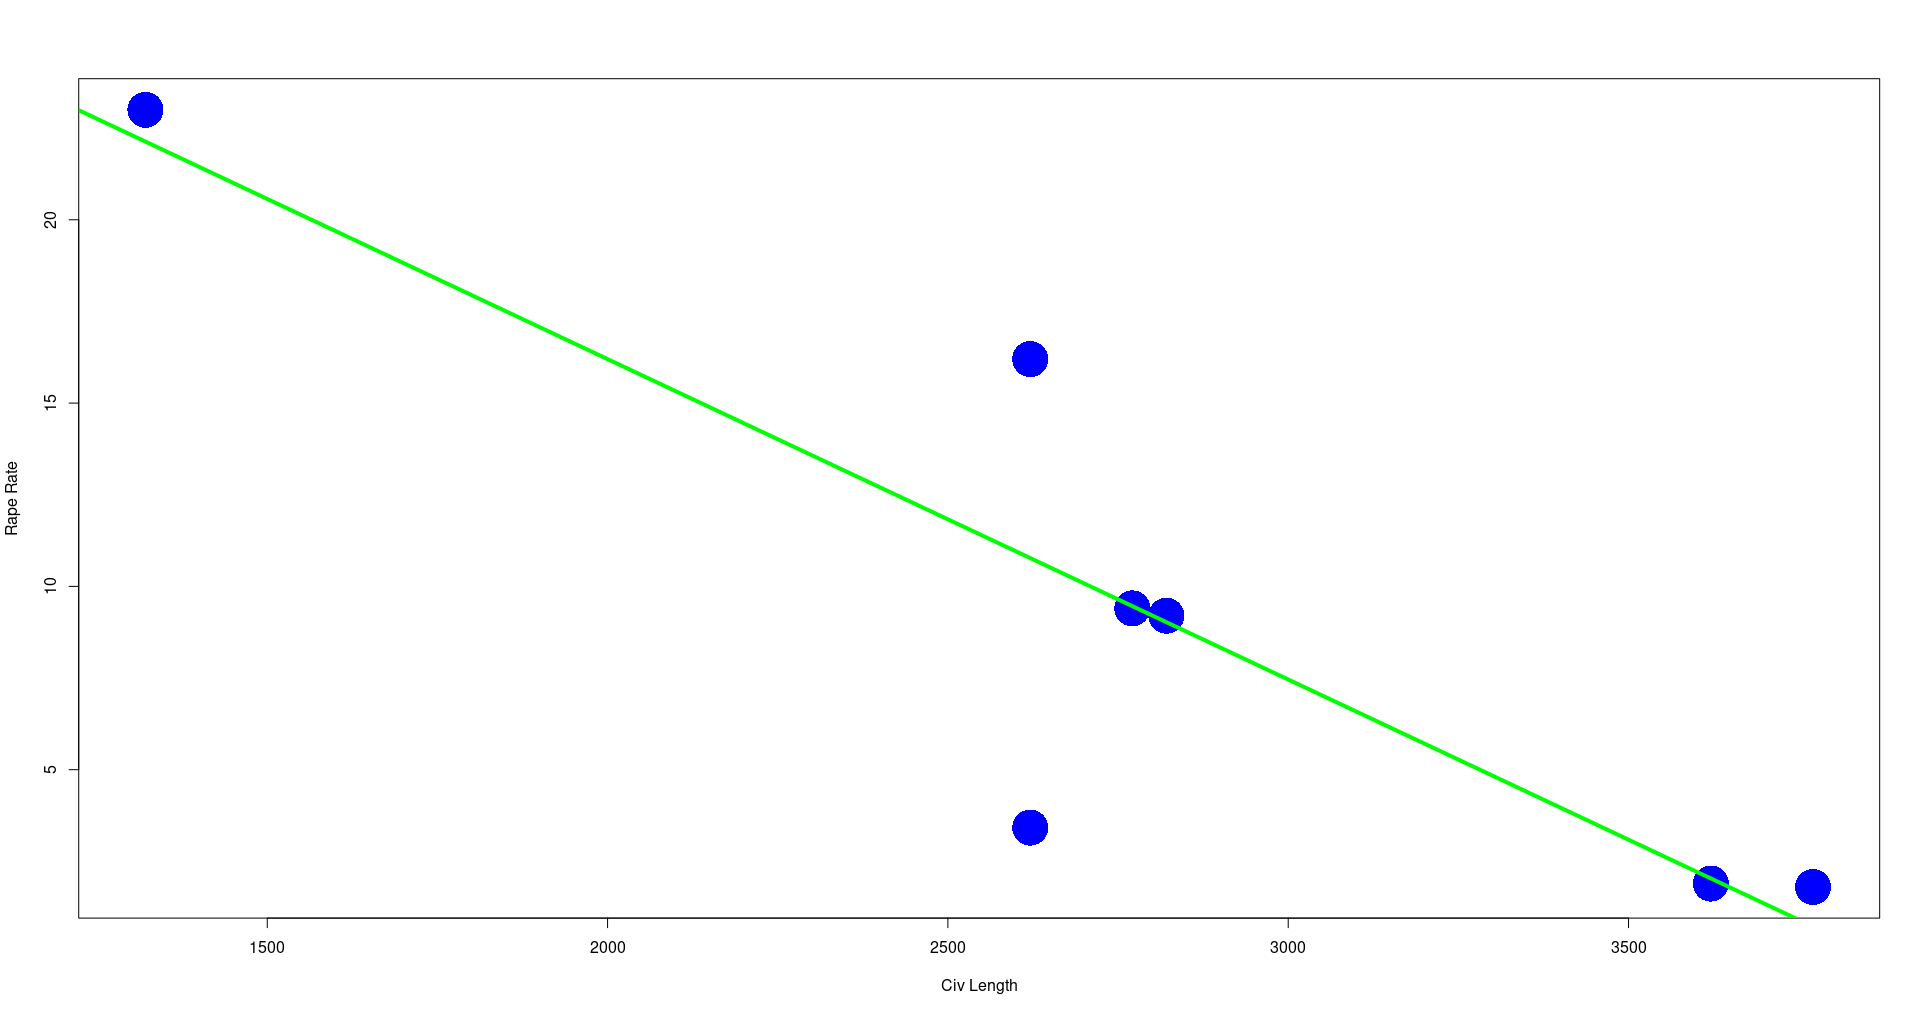
\includegraphics[scale=0.25]{rcl.jpg}

The data includes Germany, India, Spain, France, Greece, etc. 
\begin{center}
	\begin{tabular}{ |c | c | c | }
	\hline
Years	& Rape Rate &	Country \\
1321 & 23 & England\\
2771 & 9.4 & Germany \\
3771 & 1.8 & India \\
3621 & 1.893 & Greece\\
2621 & 3.42 & Spain\\
2621 & 16.2 & France\\
2821 & 9.2 & Netherlands \\
	\hline
	\end{tabular}
\end{center}


The model fit information follows.

\begin{verbatim}
> rt<-rapetimes
> mod<-lm(rt$rapes~rt$t)
> summary(mod)

Call:
lm(formula = rt$rapes ~ rt$t)

Residuals:
       1        2        3        4        5        6        7 
 0.86742 -0.06056  1.07877 -0.13913 -7.35146  5.42854  0.17641 

Coefficients:
             Estimate Std. Error t value Pr(>|t|)   
(Intercept) 33.677225   6.074272   5.544  0.00262 **
rt$t        -0.008739   0.002102  -4.158  0.00885 **
---
Signif. codes:  0 ‘***’ 0.001 ‘**’ 0.01 ‘*’ 0.05 ‘.’ 0.1 ‘ ’ 1

Residual standard error: 4.135 on 5 degrees of freedom
Multiple R-squared:  0.7756,	Adjusted R-squared:  0.7308 
F-statistic: 17.29 on 1 and 5 DF,  p-value: 0.008845
\end{verbatim}

\section{Conclusion}
There are many ethnicity based or other sorts of theories that are popular for rape rates.  Those theories are not good science.  Our theory is much better science.  The explanation is clear and parsimonious, that the influence of long contiguous civilization led to natural selection removing rapists genes from propagating.  

\begin{thebibliography}{CCC}
\bibitem{RS}{\url{https://www.nationmaster.com/country-info/stats/Crime/Rape-rate}}
\end{thebibliography}
\end{document}